In order to explore the profile of the string, we solve the non-linear system of second order differential equations for the fields $\phi$, $\xi$ and $a$, 
\begin{equation}
	\partial_r^2 \phi + \frac{1}{r} \partial_r \phi- \frac{1}{r^2}\left(n^2+2nha+h^2a^2\right)\phi- m^2 \phi- \lambda \phi^3-\kappa \phi \xi^2 = 0,
\end{equation}
\begin{equation}
	\partial_r^2 \xi + \frac{1}{r} \partial_r \xi - \frac{1}{r^2}\left(n'^2+2n'h' a+h'^2a^2 \right)\xi -m'^2\xi - \lambda' \xi^3 - \kappa \xi \phi^2 = 0 ,
\end{equation}
\begin{equation}
	\partial_r^2a -\frac{1}{r}\partial_r a-hn\phi^2-h^2a\phi^2-h' n'\xi^2 - h'^2 a \xi^2 = 0.  
\end{equation}
When $n,n'\neq 0$, they are subject to the boundary conditions, derived in Chapter 3,
\begin{eqnarray}
	\phi(0)=0, & \displaystyle\lim_{r\to\infty}\phi(r) = v, \nonumber \\
	 \xi(0)=0, &  \displaystyle\lim_{r\to\infty}\xi(r) = v', \nonumber  \\
	 a(0)=0, & \displaystyle \lim_{r\to\infty}a(r) = -\frac{n}{h}=-\frac{n'}{h'},
\end{eqnarray}
and
\begin{align}
	\label{eq:constraints}
	\lambda>0, \ \ \ \lambda'>0, \ \ \ \kappa^2 < \lambda \lambda',\nonumber \\
	 m^2 = -\kappa v'^2 - \lambda v^2<0,\ \ \ m'^2 = -\kappa v^2 - \lambda' v'^2<0. 
\end{align}

The solutions to the boundary value problem are obtained numerically by the Python function \texttt{scipy.integrate.solve\_bvp} which applies the damped Newton method.
The Newton method is a procedure of solving systems of ordinary differential equations where an initial guess is generated and subsequent iterations of the method give, ideally,  better ap\-prox\-i\-ma\-tions to the solution.

Let us take a vector function $\vec{f}(\vec{x})$ and let $\vec{x}^*$ be a root, i.e.\ $\vec{f}(\vec{x}^*)=0$. If we choose an initial guess $\vec{x}_0$ for the root, the method gives a sequence of approximations $\vec{x}_{1},\, \vec{x}_{2},\dots,\, \vec{x}_{n+1}$ by solving the system of equations
\begin{equation}
	J(\vec{x}_n)\vec{\xi} = - \vec{f}(\vec{x}_n), 
\end{equation}
where $J(\vec{x}_n)$ is the Jacobian matrix and the Newton direction $\vec{\xi}$ is defined through $\vec{x}_{n+1} = \vec{x}_{n}+\vec{\xi}$.
An ap\-prox\-i\-ma\-tion is generated by the previous one in the Newton direction. The length of the Newton direction is called the step size. In some situations, the Newton step size is too large, so we require it to be smaller. The idea of the damped Newton method is to modify the length of the Newton step size in order to have better convergence in some situations. Thus, we modify the solution by
\begin{equation}
	\vec{x}_{n+1} = \vec{x}_{n} + \lambda\vec{\xi}, \ \ \ 0<\lambda\leq 1.
\end{equation} 
See Ref.\ \cite{Ascher} for a complete review on this topic.

 A solution is uniquely defined by inputting the values for the Higgs expectation values $v$, $v'$, the self-coupling constants $\lambda$, $\lambda'$, the Higgs fields interaction term $\kappa$, the coupling constants $h$, $h'$ and finally the winding numbers $n$ and $n'$ subject to the constraints in eq.\ \eqref{eq:constraints}. We choose $v'>v$ in order to have a heavier $\chi$ boson than the standard Higgs field $\Phi$. Also, $v=246$ GeV is used to convert all quantities into physical units.  For instance, lengths are converted into physical units through
\begin{equation}
	r_{\text{physical}} = r_{\text{dimensionless}} \ \ \frac{v_{\text{dimensionless}}}{246 \ \text{GeV}} \ \ 0.197 \ \text{GeV} \ \text{fm}.
\end{equation}

Figure \ref{fig:fig1} shows the case $n=n'=h=h'=\lambda=\lambda'=1$, $v = 0.5$, $v'=1$ (in units where $v=246$ GeV) and $-1<\kappa<1$. We see the typical profile behavior of cosmic strings. Approximately at $r \gtrsim 7.5$ which corresponds to  $0.003\ \text{fm}$, the field profiles attain their asymptotic vacuum expectation values. Solutions for positive values of $\kappa$ tend to stay closer to each other under variation  of $\kappa$ than the ones with $\kappa<0$, which spread out when $\kappa$ approaches its minimum $\kappa\to-\sqrt{\lambda\lambda'}$.

Figure \ref{fig:fig2} shows the case where $n=h=\lambda=\lambda'=1$, $n'=h'=2$, $v=0.5$, $v'=1$. We consider a higher winding number $n'$ than in the previous case and we see interesting features. We observe that the standard Higgs field exceeds, or overshoots, its vacuum expectation value at large $r$. This is an interesting phenomenon not reported in the literature.  Physically, it means that a particle passing close to the string could temporarily acquire a greater mass than far from it.
The solutions to the function $\phi$ appear to be spread out when $\kappa^2\to \lambda\lambda'$, and denser when $\kappa\to 0$. The solutions to the function $\xi$ overlap, suggesting that there exist at least two equal or very similar solutions, one with $\kappa>0$ and the other with a negative $\kappa$.%, where $\kappa\approx 0$. 

%Similar interpretations to solutions in figs.\ \ref{fig:fig3} and .
In Figure \ref{fig:fig3} we change the parameters to $n=n'=1,\ \lambda=0.5,\  \lambda'=1$, $n'=h'=0.5$, $v=0.5$, $v'=1$. We see a milder effect of the spreading of the solutions of the functions $\phi$ and $\xi$ and no overshooting.

In Figure \ref{fig:fig4} the parameters are $n=h=\lambda=\lambda'=1$, $n'=2,\ h'=1$, $v=0.5$, $v'=1.5$. We see again the overshoot of the function $\phi$, which can be associated to a greater winding number of the non-standard Higgs field, $n'>n$. % However, the peak of $\xi$ is not as high as the case in fig.\ \ref{fig:fig2}, which we associate to smaller values of the gauge couplings $h$ and $h'$.

The opposite of the previous cases appears when $n<n'$ and $h>h'$. Now the field that overshoots its vacuum expectation value is $\xi$. This means that when a right-handed neutrino passes near the string core it will acquire a greater mass than far from the string. In Figure \ref{fig:n-5h5np-1hp1l1lp1v05vp2} we see a mild overshoot in the $\xi$ function, and a overlap in the function $\phi$, in addition, a mild overlap of $a$ is visible. We also see a plateau of $\phi$ around zero, this is because the expansion of the function around the origin is proportional to $r^{|n|}$, as we saw in Chapter \ref{chap:back}.


We can include our model into a larger gauge group. According to Ref.\ \cite{Fritzsch75}, our model is embedded into the group SO(10), a Grand Unification Theory, actually the most popular since SU(5) has been ruled out. Ref.\ \cite{BUCHMULLER1991395} investigates a gauge group embedded in SO(10), namely, the gauge group $\text{SU}(3)_c\times \text{SU}(2)_L\times\text{U}(1)_Y \times \text{U}(1)_{Y'}$. The model is an extension of the Standard Model where a neutral vector boson $Z'$ is added. 
Here the non-standard hypercharge takes the form
\begin{equation}
	\label{eq:refhypercharge}
	Y' = Y - \frac{5}{4}(B-L),
\end{equation}
in contrast to the form of our hypercharge $Y'$
\begin{equation}
	Y' = 2hY - \frac{h'}{2}(B-L).
\end{equation}
Equation \eqref{eq:refhypercharge} constrains the values for the gauge couplings, so they become $h = 1/2$ and $h'= -5/2$. This also implies a condition on the winding numbers, as anticipated in eq.\ \eqref{eq:goodlimit},
\begin{equation}
	n' = -5n.
\end{equation}
We do not discuss at depth this model, we only give numerical solutions for this particular case where the gauge couplings are held fixed.

In Figure \ref{fig:fig5} with $n=1,\ n'=-5,\ h=1/2,\ h'=5/2,\ \lambda=\lambda'=1$, $v = 0.5$, $v'=1$ and $-1<\kappa<1$, we see a dramatic overshoot of the field $\phi$ when $r\sim 2.5$, it reaches almost the double of its vacuum expectation value at $r\to\infty$. However, the behavior of the function $a(r)$ does not change significantly in comparison to the previous cases. 

Figure \ref{fig:fig6} with $n=-2,\ n'=10,\ h=1/2,\ h'=-5/2,\ \lambda=\lambda'=1$, $v = 0.5$, $v'=1$ is another example within the SO(10) model. Again, the overshoot of $\phi$ is clearly visible. Here, the function $\xi$ has a flat part around zero, since the function is proportional to $r^{|n|}$, as we saw in eq.\ \eqref{eq:fapproxsol}. We add that solutions with high winding numbers can hardly be stable. 

In Refs.\ \cite{victor2022} and \cite{bietenholz2022} similar plots were reported, however they did not observe the coaxial behavior of some solutions. In the limit $v\ll v'$ and $n < n'$, we observed coaxial string solutions in the profile of $\phi$. Figure \ref{fig:coaxial} with $n=-2,\ n'=10,\ h=1/2,\ h'=-5/2,\ \lambda=\lambda'=1$, $v = 0.01$, $v'=1$, the parameters are the same as in the previous case but with a different $v$. We observe an overshoot when $\kappa \simeq 0.25$ and when $\kappa$ is grater than this value, the solution has a coaxial behavior. A coaxial solution is negative at low $r$, passes the $r$-axis, and then approaches its positive vacuum expectation value. According to Ref.\ \cite{bogo1975}, for only one Higgs field with $|n|>1$ and $2\lambda/h^2 > 1$, the interpretation of the coaxial solution is that the cosmic string is not stable. 

We also plot the energy density of the function in Figure \ref{fig:edencoaxial}. In the case $v'\gg v$, we expect a tension of the string of the order of $v'^2$. In this case $v' = 100v$, and we expect a tension of the order of $10^9 \ \text{GeV}^2$. In fact, integrating numerically the energy density, we obtain a tension $\mu$ near $1.2\times 10^{10}\ \text{GeV}^2$ for all $\kappa$-values. And its gravitational coupling is approximately
\begin{equation}
	G\mu \approx 8.3\times 10^{-29}.
\end{equation}

 This type of cosmic string with the length of an horizon would have a mass of $\sim 10^{25}$ kg, equivalent to the mass of the Earth, or five orders of magnitude smaller that the mass of the Sun. The small gravitational coupling makes it very difficult for gravitational detection, like gravitational waves or gravitational lensing. However, they are not rule out by constraints in the tension from current data.

\begin{figure}
	\centering
	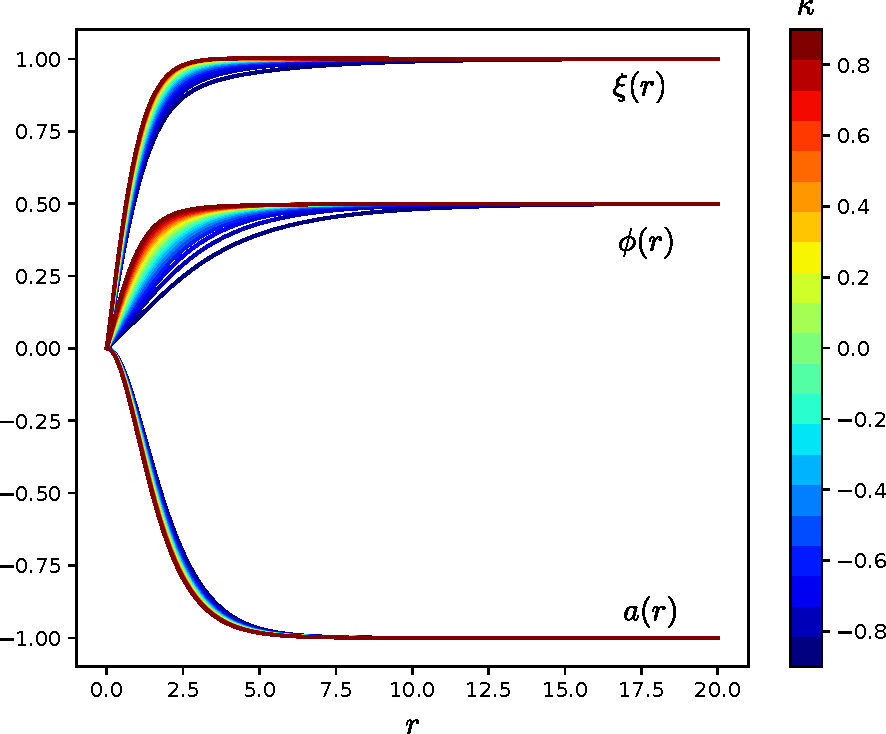
\includegraphics[scale=1]{./figures/F0.pdf}
	\caption{Solutions for the cosmic string profile functions with $v = 0.5$, $v'=1$, $n=n'=h=h'=\lambda=\lambda'=1$. Solutions with $\kappa>0$ tend to stay closer to each other, in contrast to solutions when $\kappa<0$, that spread out $\kappa$ is varied.}
	\label{fig:fig1}
\end{figure}


\begin{figure}
	\centering
	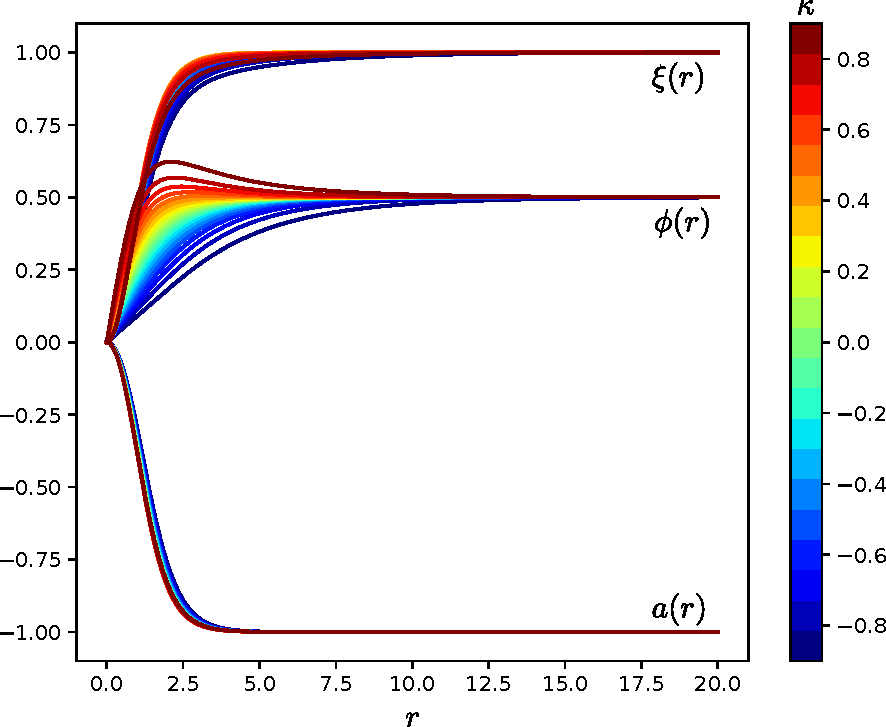
\includegraphics[scale=1]{./figures/Figure_1.pdf}
	\caption{Solutions for the cosmic string profile functions with $v = 0.5$, $v'=1$, $n=1$, $n'=2$, $h=1$, $h'=2$, $\lambda=\lambda'=1$. A lump in the profile of $\Phi$ is present. This behavior is not reported in the literature. Physically, a particle passing near the string core could acquire a greater mass than far from the string. Solution for $\xi$ overlap, which suggests that there exist very similar solutions, one with $\kappa>0$ and one with $\kappa < 0$.}
	\label{fig:fig2}
\end{figure}

\begin{figure}
	\centering
	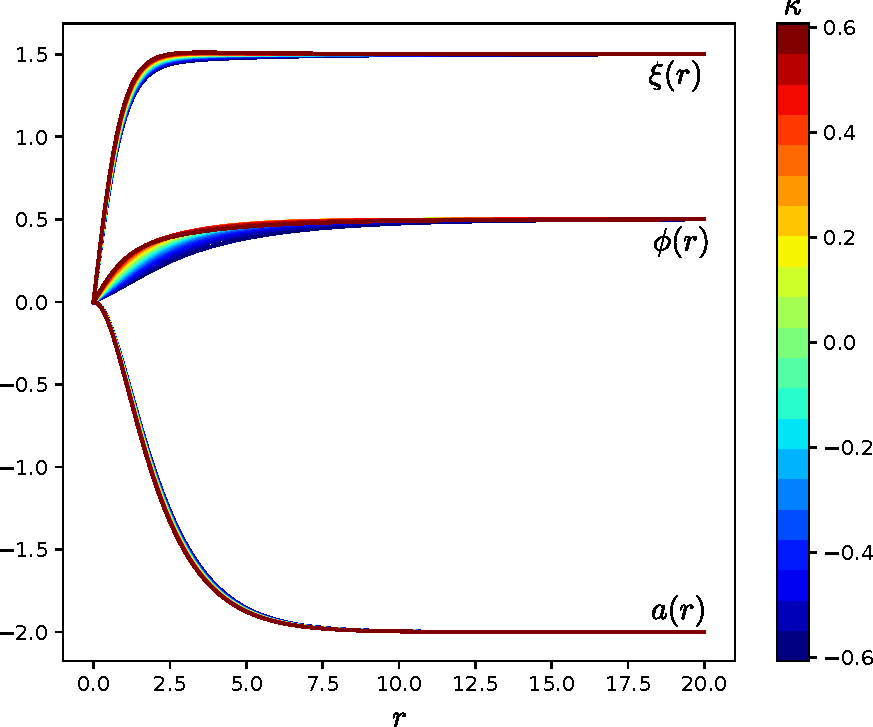
\includegraphics[scale=1]{./figures/Figure_2.pdf}
	\caption{Solutions for the cosmic string profile functions with $v = 0.5$, $v'=1$, $n=1$, $n'=1$, $h=0.5$, $h'=0.5$, $\lambda=0.5,$ $\lambda'=1$. A modest effect of the spreading in the solutions for $\phi$ is observed.}
	\label{fig:fig3}
\end{figure}


\begin{figure}
	\centering
	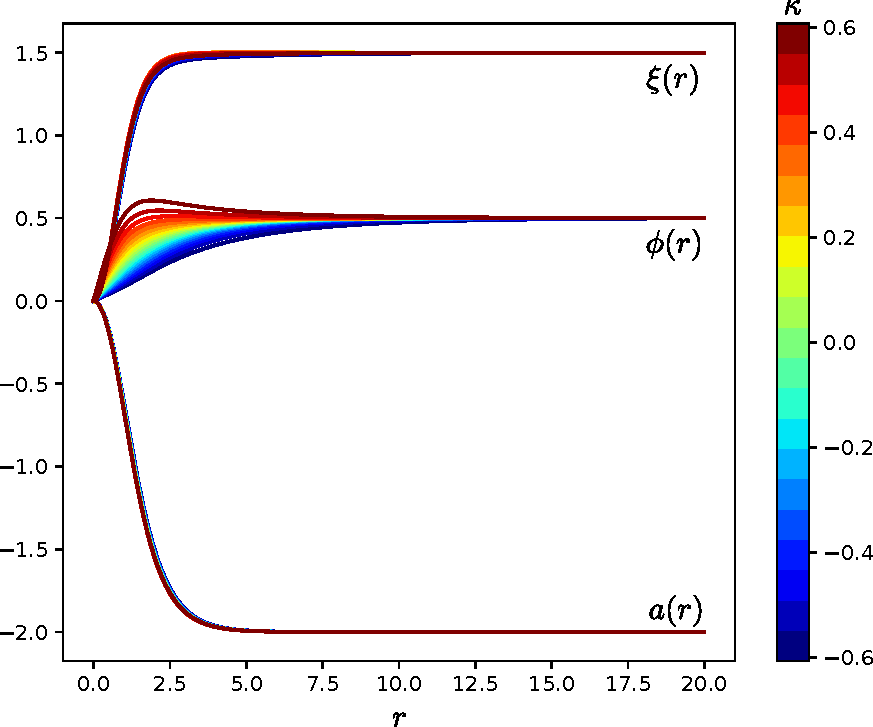
\includegraphics[scale=1]{./figures/Figure_3.pdf}
	\caption{Solutions for the cosmic string profile functions with $v = 0.5$, $v'=1$, $n=1$, $n'= 2$, $h=0.5$, $h'=1$, $\lambda=0.5,\lambda'=1$.  A lump in the profile of $\Phi$ is present. This behavior is not reported in the literature. Physically, a particle passing near the string core could acquire temporarily a greater mass than far from the string.}
	\label{fig:fig4}
\end{figure}

\begin{figure}
	\centering
	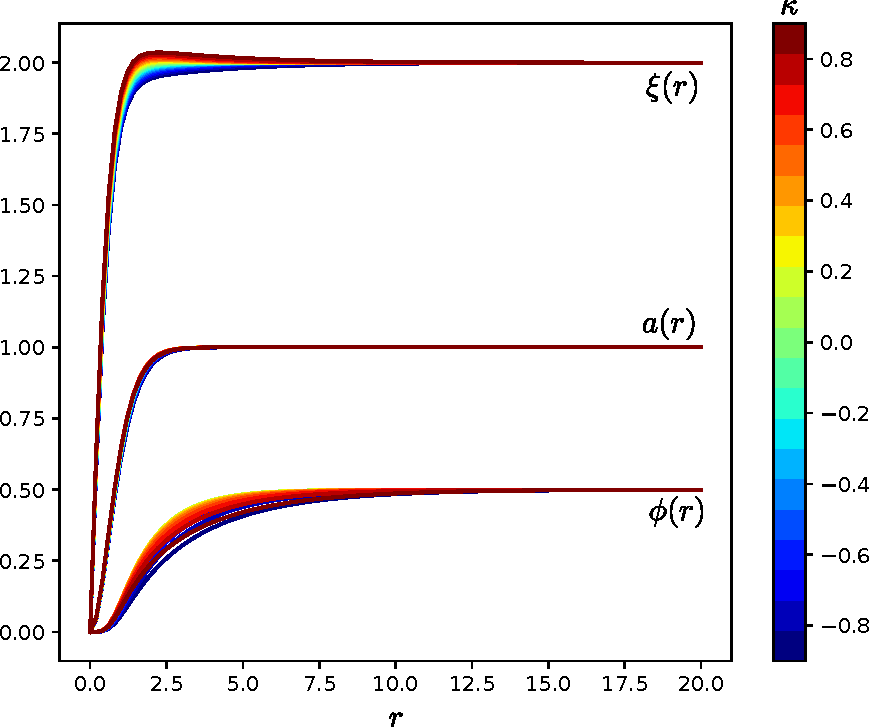
\includegraphics[scale=1]{./figures/n-5h5np-1hp1l1lp1v05vp2.pdf}
	\caption{Solutions for the cosmic string profile functions with $v = 0.5$, $v'=2$, $n=-5$, $n'=-1$, $h=5$, $h'=1$, $\lambda=\lambda'=1$. A lump in the profile of $\chi$ is present. Physically, a right-handed neutrino passing near the string core could acquire temporarily a greater mass than far from the string. This is an example from the SO(10) model.}
	\label{fig:n-5h5np-1hp1l1lp1v05vp2}
\end{figure}

\begin{figure}
	\centering
	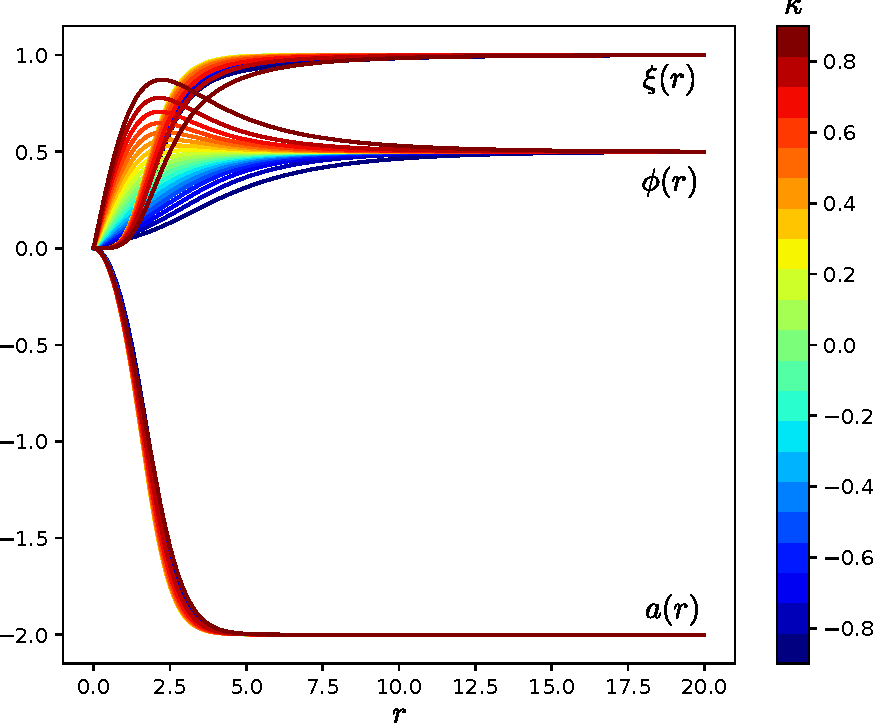
\includegraphics[scale=1]{./figures/F2.pdf}
	
	\caption{Solutions for the cosmic string profile functions with $v = 0.5$, $v'=1$, $n=1$, $n'=-5$, $h=0.5$, $h'=-2.5$, $\lambda=\lambda'=1$. This represents another example within the SO(10) GUT model. The overshoot of the field $\phi$ is clearly visible. Around $r=0$ the field $\xi$ is flat since in this region the solution is proportional to $r^{|n'|}$.}
	\label{fig:fig5}
\end{figure}

\begin{figure}
	\centering
	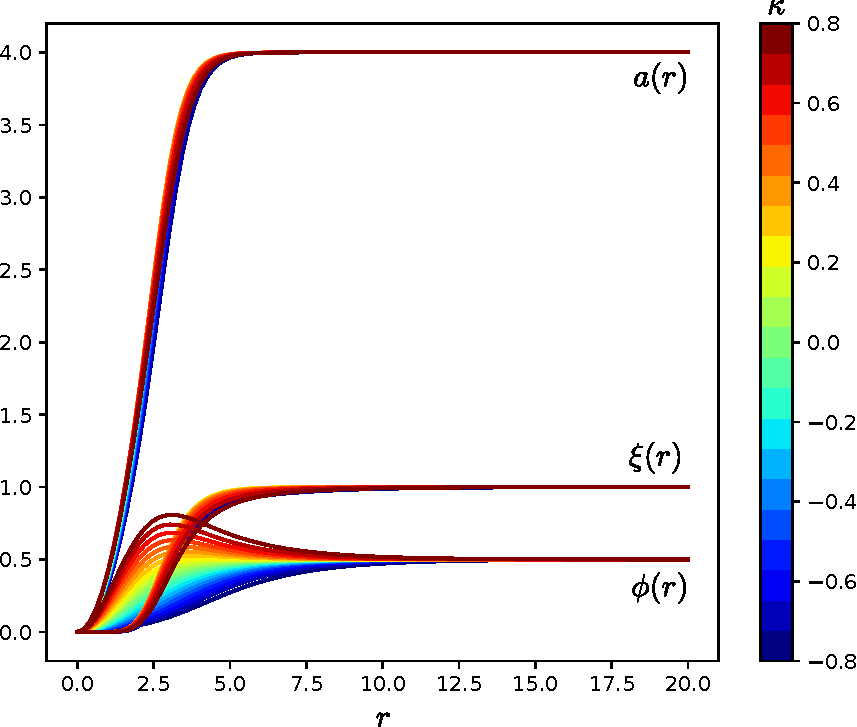
\includegraphics[scale=1]{./figures/F3.pdf}
	\caption{Solutions for the cosmic string profile functions with $v = 0.5$, $v'=1$, $n=-2$, $n'=10$, $h=0.5$, $h'=-2.5$, $\lambda=\lambda'=1$. This is another example within the SO(10) model. The overshoot of the field $\phi$ is clearly visible. Around $r=0$ the field $\xi$ is flatter than the previous case since the solution is proportional to $r^{|n'|}$.}
	\label{fig:fig6}
\end{figure}

%\begin{figure}
%	\centering
%	\begin{tikzpicture}[spy using outlines={magnification = 6, circle, size=6cm,black,connect spies}]	
%	\node (n1) at (0,0) {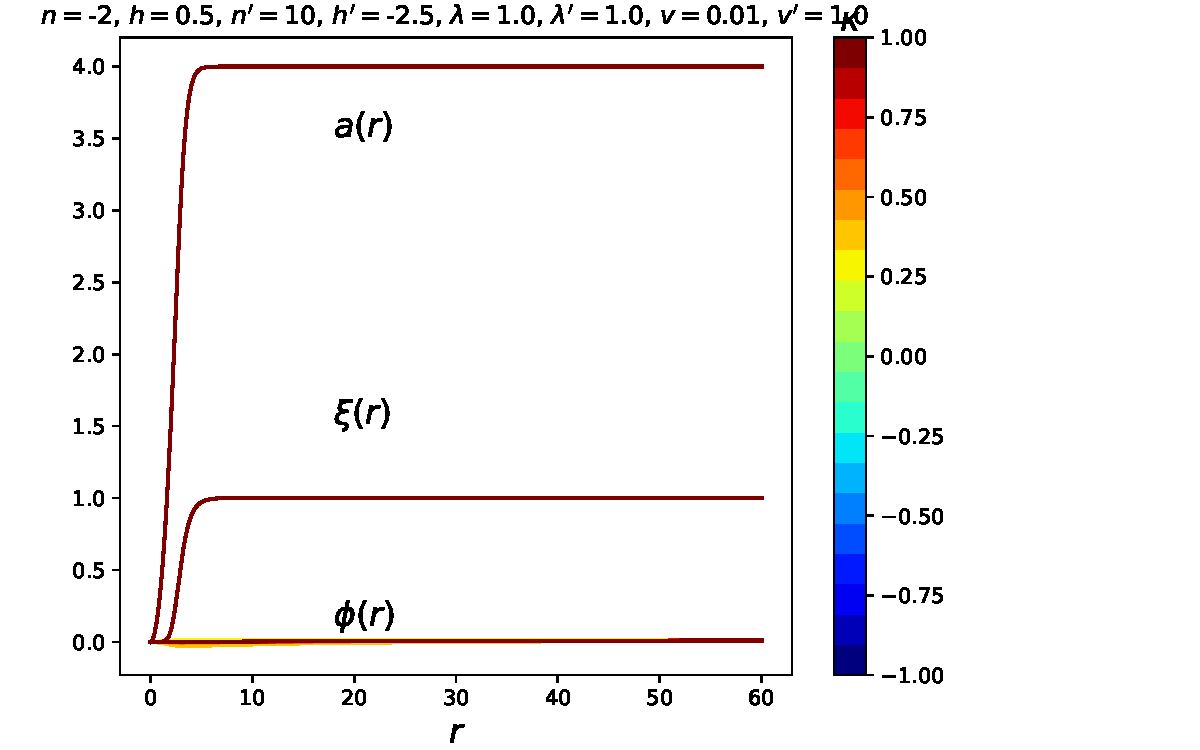
\includegraphics[scale=1]{./figures/n-2h05np10hp-25l1lp1v001vp1.pdf}};
%	\spy on (-7,-4.5) in node at (0,1);
%	\end{tikzpicture}
%\end{figure}

%\begin{figure}
%	\centering
%	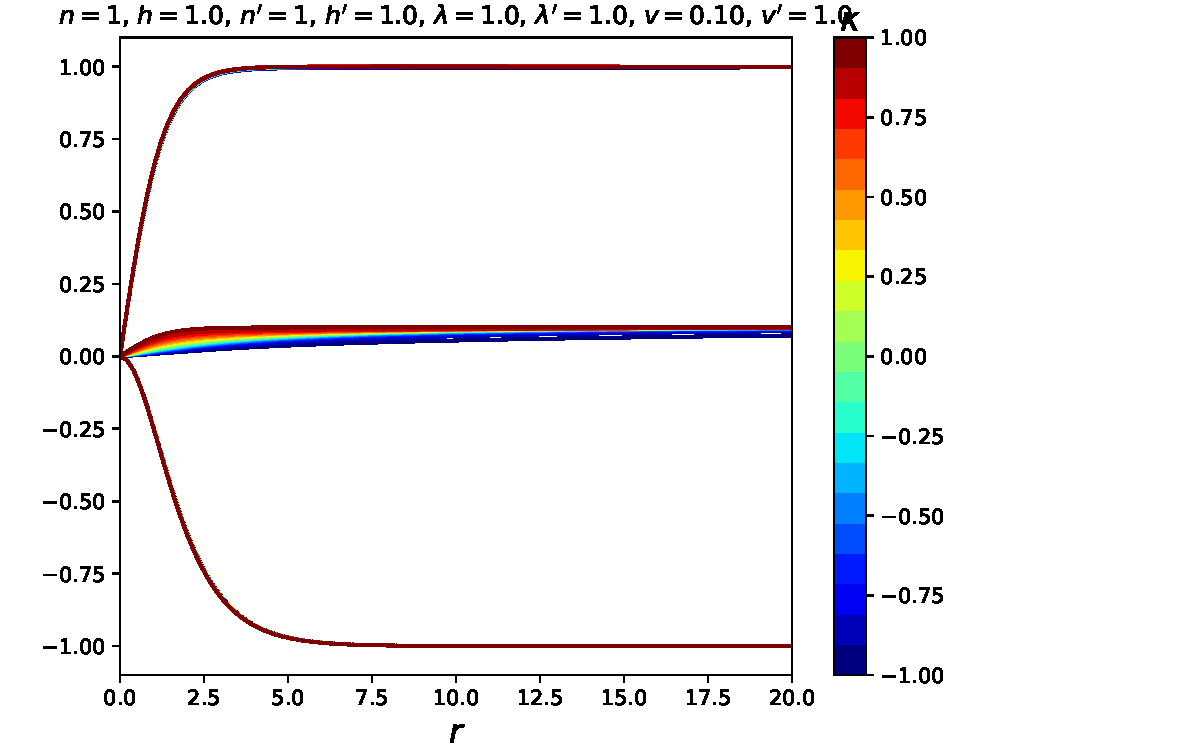
\includegraphics[scale=1]{./figures/n1h1np1hp1l1lp1v01vp1.pdf}
%	\caption{Solutions for the cosmic string profile functions with $v = 0.01$, $v'=1$, $n=-2$, $n'=10$, $h=0.5$, $h'=-2.5$, $\lambda=\lambda'=1$. Coaxial string solutions are found in a range with $\kappa>0$. A possible interpretation of the coaxial solutions regards the instability of such string with a high winding number.}
%	\label{fig:coaxial}
%\end{figure}
%
%
%\begin{figure}
%	\centering
%	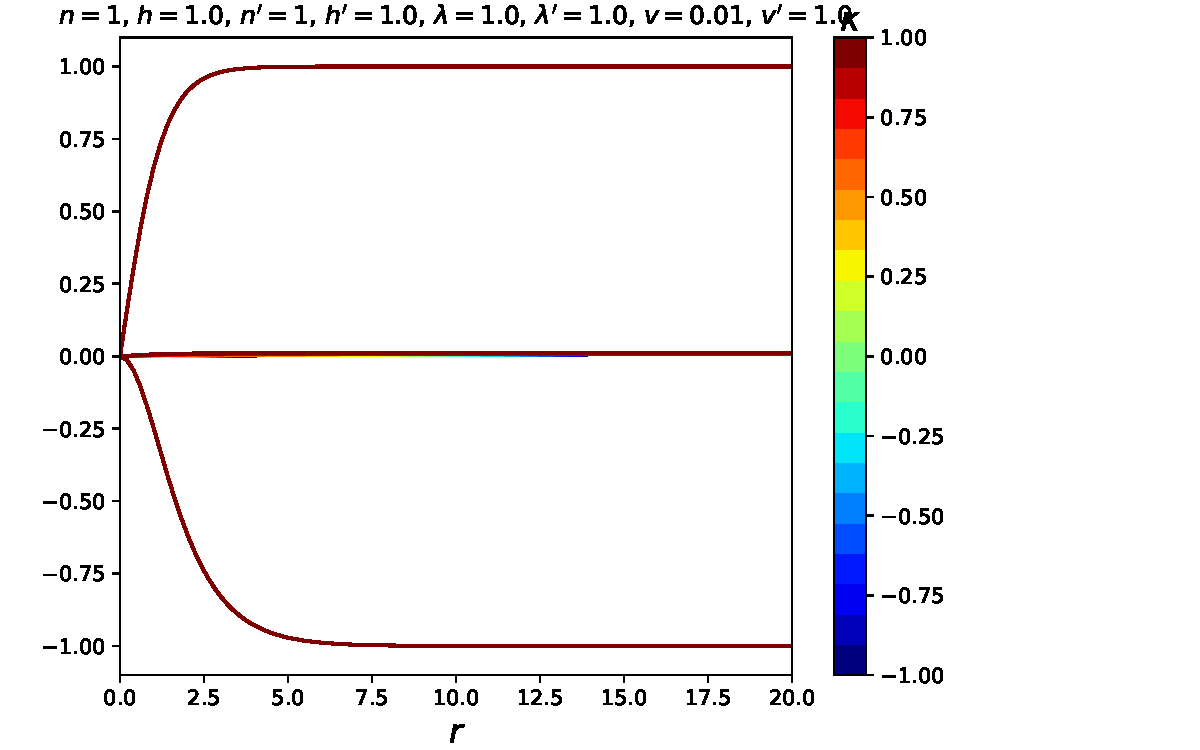
\includegraphics[scale=1]{./figures/n1h1np1hp1l1lp1v001vp1.pdf}
%	\caption{Solutions for the cosmic string profile functions with $v = 0.01$, $v'=1$, $n=-2$, $n'=10$, $h=0.5$, $h'=-2.5$, $\lambda=\lambda'=1$. Coaxial string solutions are found in a range with $\kappa>0$.}
%	\label{fig:coaxial}
%\end{figure}

\begin{figure}
	\centering
	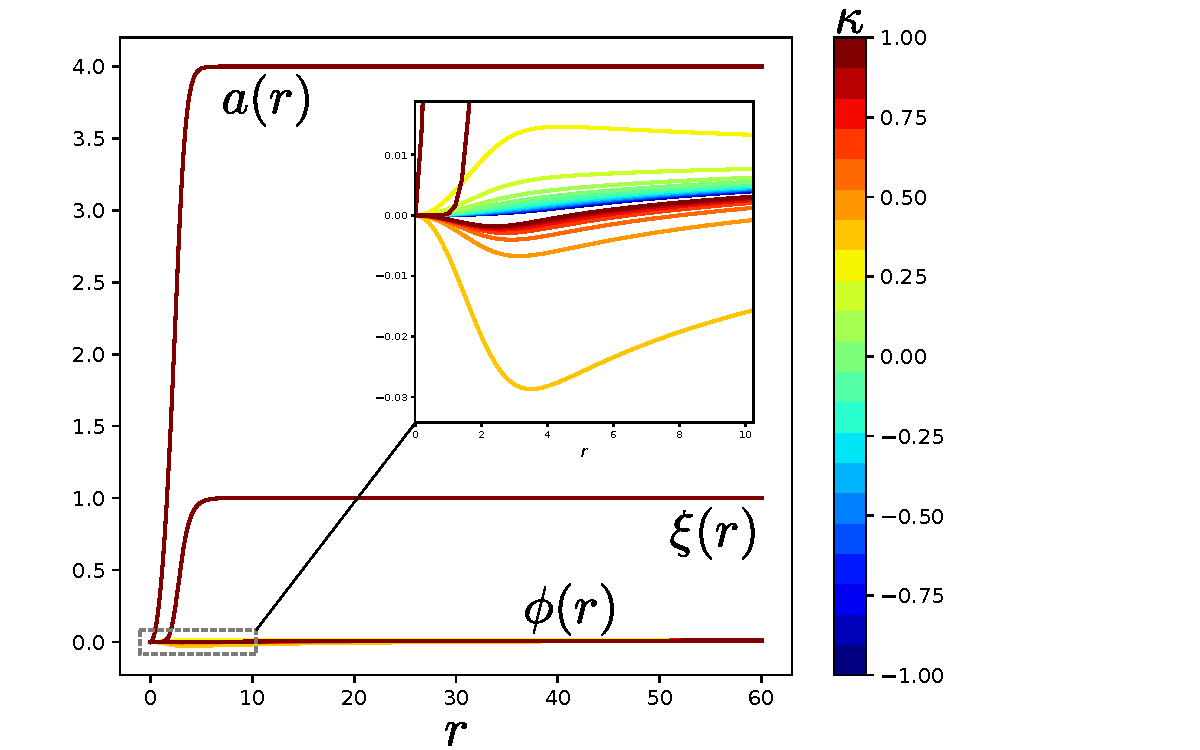
\includegraphics[scale=1]{./figures/n-2h05np10hp-25l1lp1v001vp1combined.pdf}
	\caption{Solutions for the cosmic string profile functions with $v = 0.01$, $v'=1$, $n=-2$, $n'=10$, $h=0.5$, $h'=-2.5$, $\lambda=\lambda'=1$. Coaxial string solutions are found in a range with $\kappa>0$.}
	\label{fig:coaxial}
\end{figure}

\begin{figure}
	\centering
	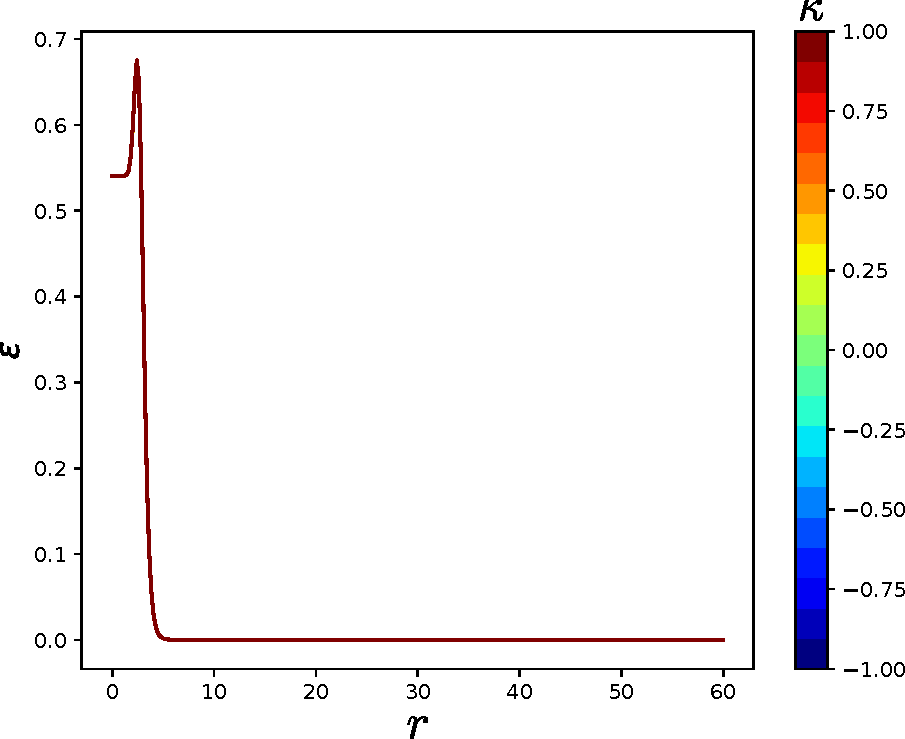
\includegraphics[scale=1]{./figures/n-2h05np10hp-25l1lp1v001vp1eden.pdf}
	\caption{Energy density of the solutions for the cosmic string profile functions with $v = 0.01$, $v'=1$, $n=-2$, $n'=10$, $h=0.5$, $h'=-2.5$, $\lambda=\lambda'=1$. The energy density is given in units of $4.79\times 10^{19}\ \text{GeV}/\text{fm}^3$.}
	\label{fig:edencoaxial}
\end{figure}

%\begin{figure}
%	\centering
%	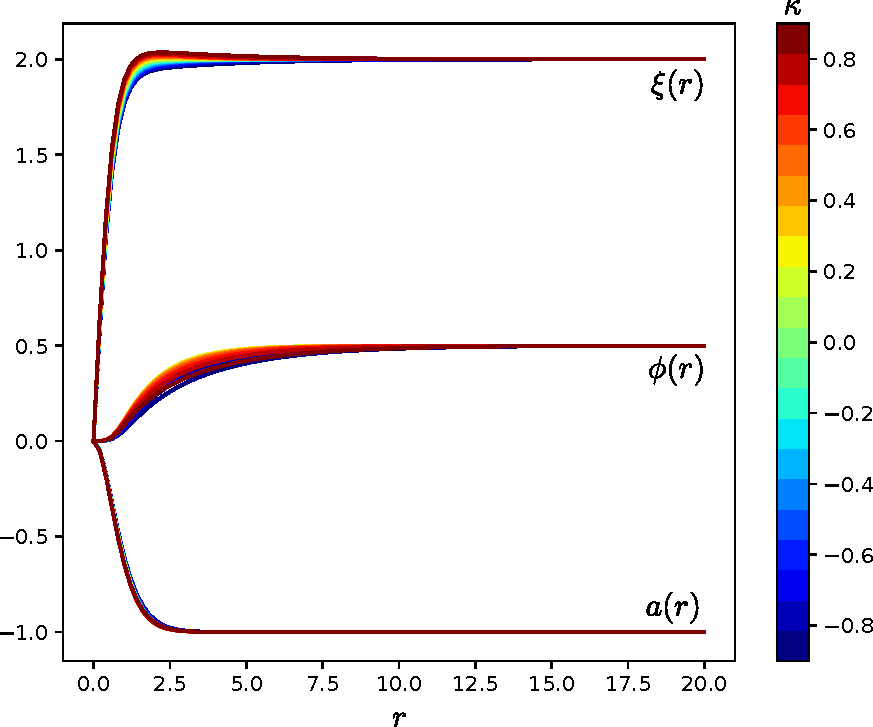
\includegraphics[scale=1]{./figures/n5h5np1hp1l1lp1v05v2.pdf}
%	\caption{Solutions for the cosmic string profile functions with $v = 0.5$, $v'=2$, $n=5$, $n'=1$, $h=5$, $h'=1$, $\lambda=\lambda'=1$.}
%	\label{fig:n5h5np1hp1l1lp1v05v2}
%\end{figure}
%
%\begin{figure}
%	\centering
%	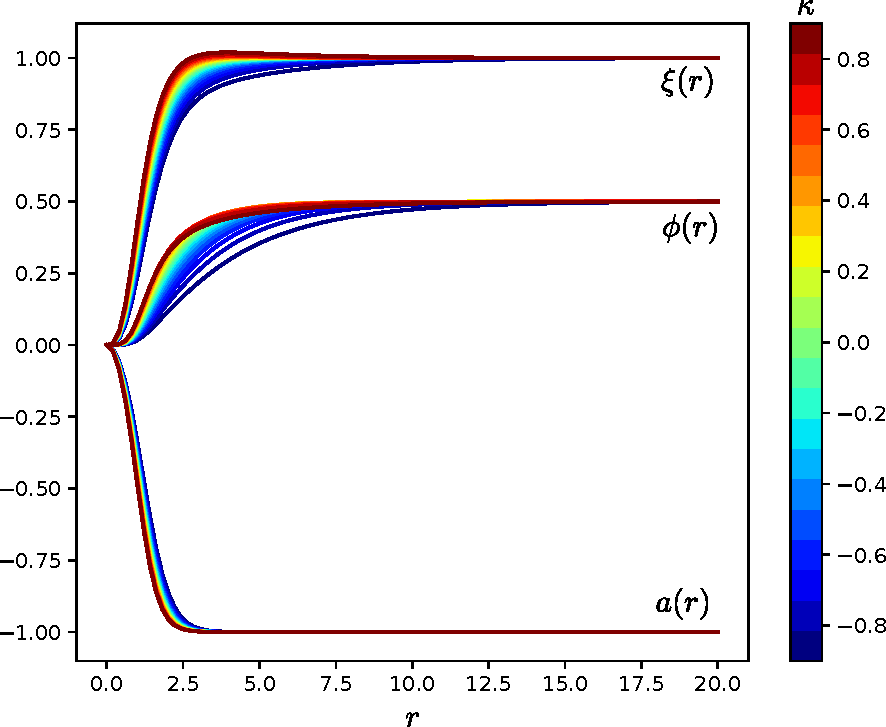
\includegraphics[scale=1]{./figures/n5h5np3h3l1lp1v05vp1.pdf}
%	\caption{Solutions for the cosmic string profile functions with $v = 0.5$, $v'=1$, $n=5$, $n'=3$, $h=5$, $h'=3$, $\lambda=\lambda'=1$.}
%	\label{fig:n5h5np3hp3l1lp1v05vp1}
%\end{figure}
%
%\begin{figure}
%	\centering
%	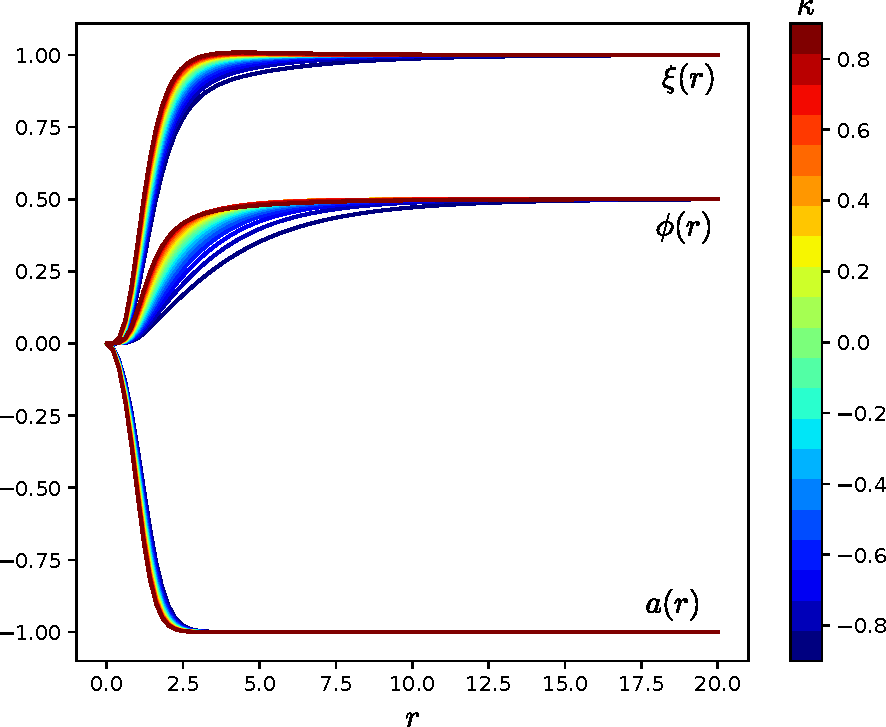
\includegraphics[scale=1]{./figures/n5h5np4hp4l1lp1v05vp1.pdf}
%	\caption{Solutions for the cosmic string profile functions with $v = 0.5$, $v'=1$, $n=5$, $n'=4$, $h=5$, $h'=4$, $\lambda=\lambda'=1$.}
%	\label{fig:n5h5np4hp4l1lp1v05vp1}
%\end{figure}

